\documentclass{beamer}\usepackage[]{graphicx}\usepackage[]{color}
%% maxwidth is the original width if it is less than linewidth
%% otherwise use linewidth (to make sure the graphics do not exceed the margin)
\makeatletter
\def\maxwidth{ %
  \ifdim\Gin@nat@width>\linewidth
    \linewidth
  \else
    \Gin@nat@width
  \fi
}
\makeatother

\definecolor{fgcolor}{rgb}{0.345, 0.345, 0.345}
\newcommand{\hlnum}[1]{\textcolor[rgb]{0.686,0.059,0.569}{#1}}%
\newcommand{\hlstr}[1]{\textcolor[rgb]{0.192,0.494,0.8}{#1}}%
\newcommand{\hlcom}[1]{\textcolor[rgb]{0.678,0.584,0.686}{\textit{#1}}}%
\newcommand{\hlopt}[1]{\textcolor[rgb]{0,0,0}{#1}}%
\newcommand{\hlstd}[1]{\textcolor[rgb]{0.345,0.345,0.345}{#1}}%
\newcommand{\hlkwa}[1]{\textcolor[rgb]{0.161,0.373,0.58}{\textbf{#1}}}%
\newcommand{\hlkwb}[1]{\textcolor[rgb]{0.69,0.353,0.396}{#1}}%
\newcommand{\hlkwc}[1]{\textcolor[rgb]{0.333,0.667,0.333}{#1}}%
\newcommand{\hlkwd}[1]{\textcolor[rgb]{0.737,0.353,0.396}{\textbf{#1}}}%
\let\hlipl\hlkwb

\usepackage{framed}
\makeatletter
\newenvironment{kframe}{%
 \def\at@end@of@kframe{}%
 \ifinner\ifhmode%
  \def\at@end@of@kframe{\end{minipage}}%
  \begin{minipage}{\columnwidth}%
 \fi\fi%
 \def\FrameCommand##1{\hskip\@totalleftmargin \hskip-\fboxsep
 \colorbox{shadecolor}{##1}\hskip-\fboxsep
     % There is no \\@totalrightmargin, so:
     \hskip-\linewidth \hskip-\@totalleftmargin \hskip\columnwidth}%
 \MakeFramed {\advance\hsize-\width
   \@totalleftmargin\z@ \linewidth\hsize
   \@setminipage}}%
 {\par\unskip\endMakeFramed%
 \at@end@of@kframe}
\makeatother

\definecolor{shadecolor}{rgb}{.97, .97, .97}
\definecolor{messagecolor}{rgb}{0, 0, 0}
\definecolor{warningcolor}{rgb}{1, 0, 1}
\definecolor{errorcolor}{rgb}{1, 0, 0}
\newenvironment{knitrout}{}{} % an empty environment to be redefined in TeX

\usepackage{alltt}
\IfFileExists{upquote.sty}{\usepackage{upquote}}{}
\begin{document}
\title{Titles}
\author{Kimberly Staudt}

\begin{frame}
  \titlepage
\end{frame}

\begin{frame}
  \frametitle{Outline}
    \tableofcontents
\end{frame}


\section{Install Libraries}
\begin{frame}[fragile]
  \frametitle{Install Libraries}

First we must install the following libraries before we can begin. 
    \begin{itemize}
      \item
\begin{knitrout}
\definecolor{shadecolor}{rgb}{0.969, 0.969, 0.969}\color{fgcolor}\begin{kframe}
\begin{alltt}
\hlkwd{library}\hlstd{(dplyr)}
\end{alltt}
\end{kframe}
\end{knitrout}
      \item
\begin{knitrout}
\definecolor{shadecolor}{rgb}{0.969, 0.969, 0.969}\color{fgcolor}\begin{kframe}
\begin{alltt}
\hlkwd{library}\hlstd{(gutenbergr)}
\end{alltt}
\end{kframe}
\end{knitrout}
    \item
\begin{knitrout}
\definecolor{shadecolor}{rgb}{0.969, 0.969, 0.969}\color{fgcolor}\begin{kframe}
\begin{alltt}
\hlkwd{library}\hlstd{(tidytext)}
\end{alltt}
\end{kframe}
\end{knitrout}
    \item
\begin{knitrout}
\definecolor{shadecolor}{rgb}{0.969, 0.969, 0.969}\color{fgcolor}\begin{kframe}
\begin{alltt}
\hlkwd{library}\hlstd{(stringr)}
\end{alltt}
\end{kframe}
\end{knitrout}
    \item
\begin{knitrout}
\definecolor{shadecolor}{rgb}{0.969, 0.969, 0.969}\color{fgcolor}\begin{kframe}
\begin{alltt}
\hlkwd{library}\hlstd{(ggplot2)}
\end{alltt}
\end{kframe}
\end{knitrout}
     \item
\begin{knitrout}
\definecolor{shadecolor}{rgb}{0.969, 0.969, 0.969}\color{fgcolor}\begin{kframe}
\begin{alltt}
\hlkwd{library}\hlstd{(wordcloud)}
\end{alltt}
\end{kframe}
\end{knitrout}
    \end{itemize}
\end{frame}


\section{Using Gutenbergr}
\begin{frame}[fragile]
  \frametitle{Using Gutenbergr}
  
Download the Dunwhich Horror with the given ID and set to the dataframe, Lovecraft
\begin{knitrout}
\definecolor{shadecolor}{rgb}{0.969, 0.969, 0.969}\color{fgcolor}\begin{kframe}
\begin{alltt}
\hlstd{Lovecraft}\hlkwb{<-}\hlkwd{gutenberg_download}\hlstd{(}\hlnum{50133}\hlstd{)}
\end{alltt}
\end{kframe}
\end{knitrout}
\end{frame}

\section{Data Mining}
\begin{frame}[fragile]
\frametitle{Using Stringr}
Once downloaded, use stringr to detect and remove all instances of the word Chapter.
\begin{knitrout}
\definecolor{shadecolor}{rgb}{0.969, 0.969, 0.969}\color{fgcolor}\begin{kframe}
\begin{alltt}
\hlstd{Lovecraft}\hlkwb{<-}\hlstd{Lovecraft}\hlopt
\hlkwd{filter}\hlstd{(}\hlopt{!}\hlkwd{str_detect}\hlstd{(Horror}\hlopt{$}\hlstd{text,}\hlstr{'CHAPTER'}\hlstd{))}
\end{alltt}


{\ttfamily\noindent\bfseries\color{errorcolor}{\#\# Error in filter\_impl(.data, quo): Evaluation error: object 'Horror' not found.}}\end{kframe}
\end{knitrout}

\end{frame}

\begin{frame}[fragile]
\frametitle{Unnest Data}

Next, Unnest the the text, and store into a dataframe. 
\begin{knitrout}
\definecolor{shadecolor}{rgb}{0.969, 0.969, 0.969}\color{fgcolor}\begin{kframe}
\begin{alltt}
\hlstd{words_df}\hlkwb{<-}\hlstd{Lovecraft}\hlopt
\hlkwd{unnest_tokens}\hlstd{(word,text)}
\hlkwd{colnames}\hlstd{(words_df)}
\end{alltt}
\begin{verbatim}
## [1] "gutenberg_id" "word"
\end{verbatim}
\end{kframe}
\end{knitrout}

\end{frame}

\begin{frame}[fragile]
\frametitle{Bing Lexicon}
Use the bing lexicon to get the positive and negative sentiments in the text.
\begin{knitrout}
\definecolor{shadecolor}{rgb}{0.969, 0.969, 0.969}\color{fgcolor}\begin{kframe}
\begin{alltt}
\hlstd{bing}\hlkwb{<-}\hlkwd{get_sentiments}\hlstd{(}\hlstr{'bing'}\hlstd{)}
\hlkwd{colnames}\hlstd{(bing)}
\end{alltt}
\begin{verbatim}
## [1] "word"      "sentiment"
\end{verbatim}
\end{kframe}
\end{knitrout}

\end{frame}

\begin{frame}[fragile]
\frametitle{Inner Join}
Use inner join to display positive and negative words in the text. 
Remove the gutenberg id tag. 
\begin{knitrout}
\definecolor{shadecolor}{rgb}{0.969, 0.969, 0.969}\color{fgcolor}\begin{kframe}
\begin{alltt}
 \hlstd{words_df}\hlkwb{<-}\hlkwd{inner_join}\hlstd{(words_df,bing)}

\hlstd{words_df}\hlopt{$}\hlstd{gutenberg_id}\hlkwb{<-}\hlkwa{NULL}
\end{alltt}
\end{kframe}
\end{knitrout}

\end{frame}

\begin{frame}[fragile]
\frametitle{Positive Words}
Use dplyr to filter and count the top 10 most frequently occuring positive words.
Then store this as a factor. 
\begin{knitrout}
\definecolor{shadecolor}{rgb}{0.969, 0.969, 0.969}\color{fgcolor}\begin{kframe}
\begin{alltt}
\hlstd{pos}\hlkwb{<-}\hlstd{words_df}\hlopt
  \hlkwd{filter}\hlstd{(sentiment}\hlopt{==}\hlstr{'positive'}\hlstd{)}\hlopt
  \hlkwd{group_by}\hlstd{(word)}\hlopt
  \hlkwd{summarize}\hlstd{(}\hlkwc{count}\hlstd{=}\hlkwd{n}\hlstd{(),}\hlkwc{sentiment}\hlstd{=}\hlkwd{first}\hlstd{(sentiment))}\hlopt
  \hlkwd{arrange}\hlstd{(count)}\hlopt
  \hlkwd{top_n}\hlstd{(}\hlnum{10}\hlstd{,}\hlkwc{wt}\hlstd{=count)}

\hlstd{pos}\hlopt{$}\hlstd{word}\hlkwb{<-}\hlkwd{factor}\hlstd{(pos}\hlopt{$}\hlstd{word,}\hlkwc{levels}\hlstd{=pos}\hlopt{$}\hlstd{word)}
\end{alltt}
\end{kframe}
\end{knitrout}

\end{frame}

\begin{frame}[allowframebreaks,fragile]
\frametitle{Negative Words}
Now, do the same thing for the 10 most frequently occuring negative words.
Store this as a factor.Lastly, use rbind to combine the negative and positive words. 
\begin{knitrout}
\definecolor{shadecolor}{rgb}{0.969, 0.969, 0.969}\color{fgcolor}\begin{kframe}
\begin{alltt}
\hlstd{neg}\hlkwb{<-}\hlstd{words_df}\hlopt
  \hlkwd{filter}\hlstd{(sentiment}\hlopt{==}\hlstr{'negative'}\hlstd{)}\hlopt
  \hlkwd{group_by}\hlstd{(word)}\hlopt
  \hlkwd{summarize}\hlstd{(}\hlkwc{count}\hlstd{=}\hlkwd{n}\hlstd{(),}\hlkwc{sentiment}\hlstd{=}\hlkwd{first}\hlstd{(sentiment))}\hlopt
  \hlkwd{arrange}\hlstd{(count)}\hlopt
  \hlkwd{top_n}\hlstd{(}\hlnum{10}\hlstd{,}\hlkwc{wt}\hlstd{=count)}

\hlstd{neg}\hlopt{$}\hlstd{word}\hlkwb{<-}\hlkwd{factor}\hlstd{(neg}\hlopt{$}\hlstd{word,}\hlkwc{levels}\hlstd{=neg}\hlopt{$}\hlstd{word)}

\hlstd{combo}\hlkwb{<-}\hlkwd{rbind}\hlstd{(pos,neg)}
\end{alltt}
\end{kframe}
\end{knitrout}

\framebreak
\end{frame}


\section{Data Visualization}
\begin{frame}[allowframebreaks,fragile]
\frametitle{Plotting}
Use ggplot to create a bar chart of the positive words. 
\begin{knitrout}
\definecolor{shadecolor}{rgb}{0.969, 0.969, 0.969}\color{fgcolor}\begin{kframe}
\begin{alltt}
\hlkwd{ggplot}\hlstd{()}\hlopt{+}
  \hlkwd{geom_bar}\hlstd{(}\hlkwc{data}\hlstd{=pos,}\hlkwd{aes}\hlstd{(}\hlkwc{x}\hlstd{=word,}\hlkwc{y}\hlstd{=count),}\hlkwc{color}\hlstd{=}\hlstr{'red'}\hlstd{,}\hlkwc{fill}\hlstd{=} \hlstr{'blue'}\hlstd{,}\hlkwc{stat}\hlstd{=}\hlstr{'identity'}\hlstd{)}\hlopt{+}
\hlkwd{coord_flip}\hlstd{()}
\end{alltt}
\end{kframe}
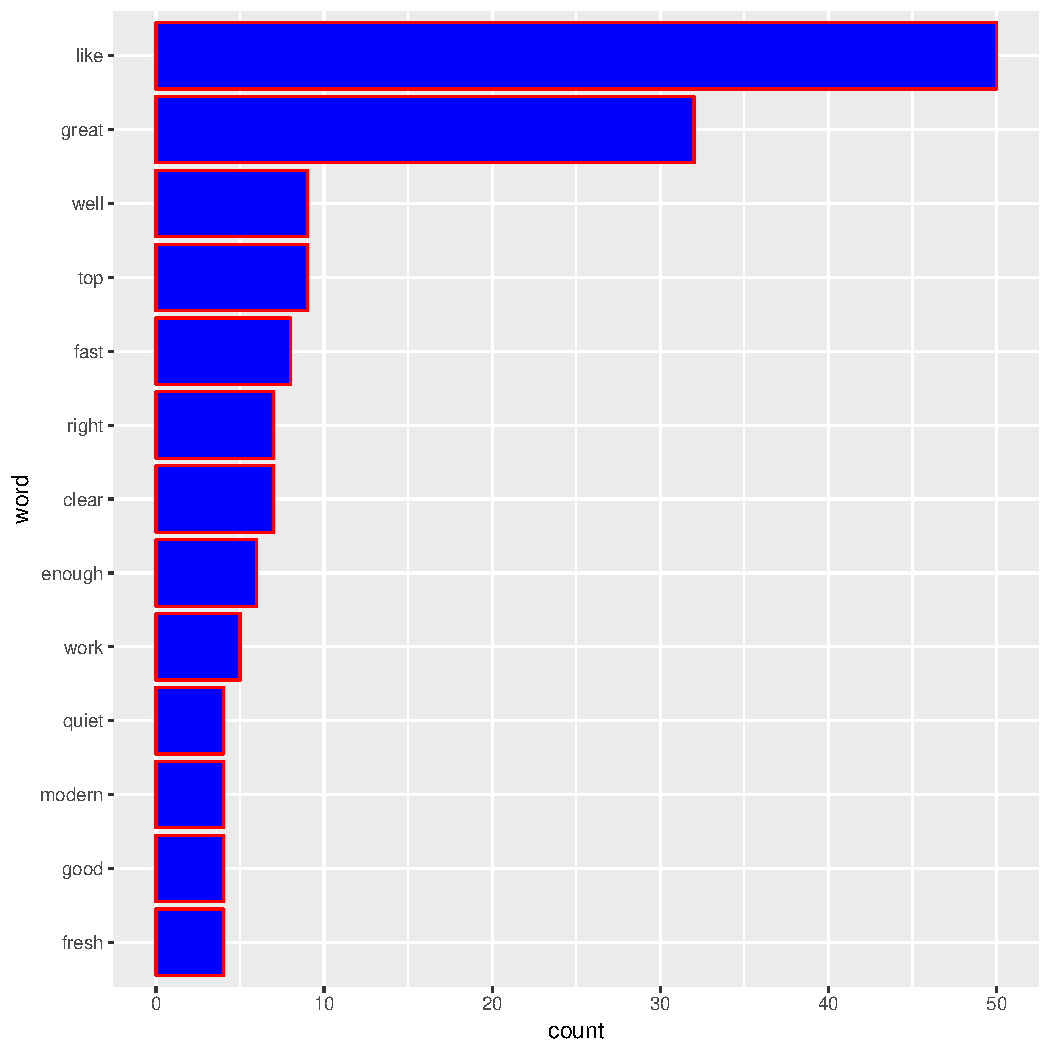
\includegraphics[width=\maxwidth]{figure/unnamed-chunk-13-1} 

\end{knitrout}
\framebreak
\end{frame}

\begin{frame}[allowframebreaks,fragile]
\frametitle{Comparing Words}
\begin{knitrout}
\definecolor{shadecolor}{rgb}{0.969, 0.969, 0.969}\color{fgcolor}\begin{kframe}
\begin{alltt}
\hlkwd{ggplot}\hlstd{()}\hlopt{+}
  \hlkwd{geom_bar}\hlstd{(}\hlkwc{data}\hlstd{=combo,}
           \hlkwd{aes}\hlstd{(}\hlkwc{x}\hlstd{=word,}\hlkwc{y}\hlstd{=count,} \hlkwc{fill}\hlstd{=sentiment,}
               \hlkwc{color}\hlstd{=sentiment),}\hlkwc{stat}\hlstd{=}\hlstr{'identity'}\hlstd{)}\hlopt{+}
  \hlkwd{coord_flip}\hlstd{()}\hlopt{+}
  \hlkwd{facet_wrap}\hlstd{(}\hlopt{~}\hlstd{sentiment,}\hlkwc{scales}\hlstd{=}\hlstr{'free_y'}\hlstd{)}\hlopt{+}
  \hlkwd{scale_fill_manual}\hlstd{(}\hlkwc{values}\hlstd{=}\hlkwd{c}\hlstd{(}\hlstr{'red'}\hlstd{,}\hlstr{'yellow'}\hlstd{))}\hlopt{+}
\hlkwd{scale_color_manual}\hlstd{(}\hlkwc{values}\hlstd{=}\hlkwd{c}\hlstd{(}\hlstr{'yellow'}\hlstd{,}\hlstr{'red'}\hlstd{))}
\end{alltt}
\end{kframe}
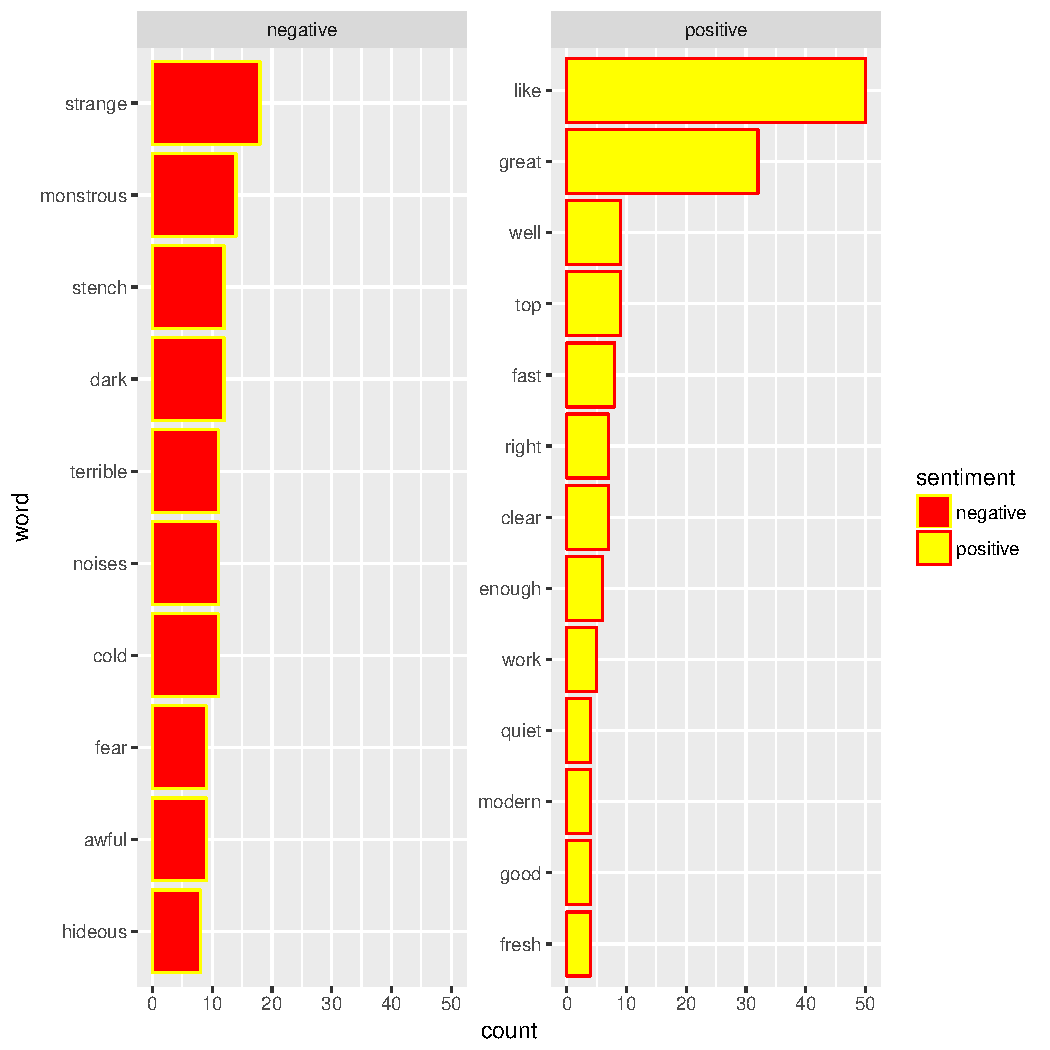
\includegraphics[width=\maxwidth]{figure/unnamed-chunk-14-1} 

\end{knitrout}
\framebreak
\end{frame}


\end{document}
